The $n$-dimensional ice cream of radius $R>1$, denoted $RI$ is the convex hull of the unit ball and the point $(R,0,0...,0)$. In this section, we will simply argue that its volume is

$$
\vol_n(RI) = \frac{R-h}{n} \vol_{n-1}(rB) + \vol_n(B) - \left(\frac{1}{2}\vol_n(rB) I_{\frac{2rh-h^2}{r^2}}\left(\frac{n+1}{2}, \frac{1}{2}\right)\right)
$$

With $h = \frac{1}{R}$, $r = \sqrt{1-\frac{1}{R^2}}$ and $I_x(a,b)$ is the incomplete beta function, defined thus:

$$
I_x(a,b) = \frac{\int^x_0 t^{a-1}(1-t)^{b-1}dt}{\int^1_0 t^{a-1}(1-t)^{b-1} dt}
$$

We will show that the shape can be written as the union of two disjoint sets. Let
$$
S = B \cap \left\{\bm{x} \in \arr^n | x_1 \leqslant \frac{1}{R}\right\}
$$
And
$$
W = \left\{\bm{x} + \left(\frac{1}{R}, 0, ..., 0\right) | x_1 > 0 \; \wedge \; \sum^{n}_{i=2} x_i^2 < \left(\frac{\sqrt{1-R^{-2}}}{R-R^{-1}} x_1\right)^2 \right\}
$$

We will call $S$ the scoop, and is the spherical part of the ice cream near the origin, and $W$ the wafer, the conical part nearer to the point $(R,...,0)$. These two shapes are clearly disjoint, so the volume of the ice cream is the sum of the volumes of the scoop and the wafer. We will show that these shapes partition the ice cream by showing that any line tangent to the unit ball through $(R,0,...,0)$ touches the ball at a point whose first coordinate is $\frac{1}{R}$.  The set of points touching the surface of an $n$-ball whose first coordinate is $\frac{1}{R}$ is an $(n-1)$-ball of radius $\sqrt{1-R^{-2}}$, and the distance from this surface to $(R,0,...,0)$ is $1-\frac{1}{R}$. The convex hull of points on an $n-1$ dimensional surface with a point normal to the surface is an $n$-dimensional hypercone. This hypercone is the wafer, the remainder is the scoop. Most of this will manifest as simple but non-obvious geometry, so it is worth describing fully.

\begin{proposition}
A line tangent to the unit $n$-ball that passes through $(R,0,...,0)$ intersects the surface of the $n$-ball at a point whose first coordinate is $\frac{1}{R}$ at a distance $\sqrt{1-\frac{1}{R^2}}$ from the line from the origin to $(R,0,...,0)$
\end{proposition}

The situation is as depicted in figure~\ref{fig_ice_cream_annotated}. $O$ is the origin, $B$ is the point $(R,0,...,0)$, and $A$ is any point on the surface of the unit $n$-ball such that $AB$ is tangent to the surface. $OAB$ is a right angle. $C$ is the point such that $O$, $C$ and $B$ are colinear, and $ACB$ is a right angle. Since $OAB$ is a right angled triangle, $|AB| = \sqrt{R^2-1}$. From the law of sines, $\sin(AOB) = \frac{\sqrt{R^2-1}}{R}$, so $\cos(AOB) = \frac{1}{R}$, so $|OC| = \frac{1}{R} = h$, and $|AC| = \sqrt{1-\frac{1}{R^2}} = r$, as required.

We also have that $|CB| = R-h$, and that the points on the surface of the unit ball whose first coordinate is $h$ is an $(n-1)$-ball of radius $r$. This tells us that the wafer is an $n$-dimensional hypercone of height $R-h$ and whose base is the $(n-1)$-ball of radius $r$.

\begin{figure}
\centering
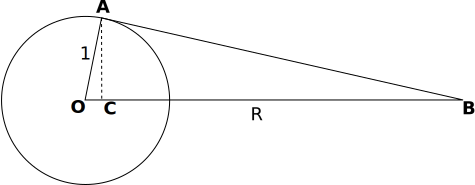
\includegraphics{./images/ice_cream_annotated.pdf}
\caption{Annotated components of an ice-cream, projected onto the 2-d plane. Points are in bold font, and variables in italic.}
\label{fig_ice_cream_annotated}
\end{figure}

\begin{proposition} \label{prop_vol_wafer}
The volume of the wafer is $\frac{R-h}{n} \vol_{n-1}(rB)$
\end{proposition}

The set of points in the wafer at a distance of $t$ from point $B$ is exactly the set of points in the $(n-1)$-ball of radius $\frac{rt}{R-h}$, so

\begin{align*}
\vol(W)
&= \int^{R-h}_{0} \vol_{n-1}\left(\frac{t}{R-h}rB\right) dt \\
&= \frac{1}{R-h}^{n-1} \vol_{n-1}(rB) \int^{R-h}_0 t^{n-1}dt \\
&= \frac{R-h}{n} \vol_{n-1}(rB)
\end{align*}
As required.

\begin{proposition} \label{prop_vol_scoop}
The volume of the scoop is $\vol_n(B) - \left(\frac{1}{2}\vol_n(rB) I_{\frac{2rh-h^2}{r^2}}\left(\frac{n+1}{2}, \frac{1}{2}\right)\right)$
\end{proposition}

The scoop is exactly a unit hypersphere without a hyperspherical dome. The volume of an $n$-spherical dome of height $h$, radius $r$ is $\frac{1}{2}\vol_n(rB) I_{\frac{2rh-h^2}{r^2}}\left(\frac{n+1}{2}, \frac{1}{2}\right)$, as proven in \cite{Li11}, so the volume of the scoop is $\vol_n(B) - \left(\frac{1}{2}\vol_n(rB) I_{\frac{2rh-h^2}{r^2}}\left(\frac{n+1}{2}, \frac{1}{2}\right)\right)$

Combining propositions~\ref{prop_vol_wafer} and~\ref{prop_vol_scoop}, we have the volume of the entire ice cream.